% !TeX spellcheck = en_GB

\subsection*{Search Terms TOTAL PAGES 18.85/69}
portal
3D lense
magic lense
Seams

dual depth buffer
Walkthrough applications
Transformative Portal
\section{Introduction 0/1}

\subsection{Disambiguation}
portal in a game
vs
portal as occlusion culling

\section{Literatur 0/15}

\subsection{Portals as Occlusion Culling}
potentially visible set
\cite{luebke:1995:portals}
\cite{yang:2014:walkthrough}

\subsection{Portals Algorithms History}


Portal Rendering in SEAMS (\cite{schmalstieg:1999:sewing})

Complex Portal rendering. (I use the same near Buffer technique) \cite{ lowe:2005:technique}


\url{https://th0mas.nl/2013/05/19/rendering-recursive-portals-with-opengl/}
\subsection{Portal Applications}

\subsubsection{Magic Lense}
\cite{viega:1996:3d}


\subsubsection{VR Interaction 3D Lenses}
\cite{borst:2009:real}
3D lenses which change, the properties. E.g. other rendered objects (x ray lense), inverted colors, fish eye effect.

\subsubsection{Navigation}
Portal Rendering in SEAMS (\cite{schmalstieg:1999:sewing})
\cite{pausch:1995:navigation} navigation with hand held minatures


\subsubsection{Game Mechanik}
Portal, Antichamber, Splitgate Warfare Arena

\subsubsection{VR Movement}

Portal Locomotion in Budget Cuts\url{https://www.youtube.com/watch?v=f786ak3GKQo}

\subsubsection{Fit More Space in Less Space}

\subsubsection{Space Division}
Rooms are split by portals. For each portal only the objects in its room need to be drawn.
\cite{ lowe:2005:technique}

\subsection{Graphics Programming 0/9}


\subsubsection{Raytracing}
software,
gpu,
NVIDIA RTX cards, Ray shaders?

\subsubsection{Rasterization}

\subsubsection{GPU Synchronisation}

\subsubsection{Uniforms / Storage Buffer Objects}

\subsubsection{Shaders / (Vulkan-) GLSL / SPIR-V}
branching, fragment discard, early stencil / depth, force early test, Stencil Export

\subsubsection{Occlusion Queries}

\subsubsection{OpenGL}
History


\subsubsection{Vulkan Overview}
input attachments, tile renderers,

(Sub-)Renderpass, Push Constants, Validation Layers, Pipelines, Dynamic state,

Molten VK-Framwork

\subsubsection{Depth / Stencil Test}
Limitations, common uses
Early Z! Fragment discard
Z Fighting,
Depth Formtas
inverse depth buffer with floating point is magic!

combined depth / stencil
\url{https://developer.nvidia.com/content/depth-precision-visualized}

\subsubsection{Push Constant}

\subsubsection{Instanced Drawing}

\section{Implementation 23.6/30}

\subsection{Technologies / Libraries}
SDL, glm, vulkan, rapid xml, c++, vulkan memory allocator

\subsubsection{debugging}
validation layers render doc


\subsection{Software Raytracing 0.5}
The first implementation was based on software raytracing. Compared to rasterization based methods, raytracing allows for more complex operations on individual rays. A response to an instersection can spawn a new ray, which replaces the old ray. The new ray can have many different properties. The new ray can have an completely different origin and direction, which would simulate a portal. Additionally a non conventional ray definition could be used, allowing for bent rays. Rays could travel slower, resulting in scaled space.

The prototype was implemented in C++ using SDL \cite{sdl} and GLM \cite{glm} as libraries. It performs an intersection test against sphere. The ray line intersection query uses the algorithm described by \textcite{eberly:2006:3d}. Additionally, the pixels of the SDL Surface were manipulated directly instead of using an SDL Renderer to improve performance.

Even with this simple test, the prototype performed poorly. A scene with only one sphere took more than 40 milliseconds to render on a 1920x1080 resolution. When subtracting the time needed to render an empty scene, it still takes over 20 milliseconds. For realtime applications it is completely unviable.

There are still some improvement opportunities with multithreading, rendering to smaller resolutions, and using simpler tests. However, with an high render time already this high, continuing seemed to risky and this approach was abandoned.

%TODO Include Measurements and PC Stats?

\subsection{Why Vulkan 0.5}
One important aspect of the prototpye was that it can run on as many plattforms as possible. %TODO: Should / Where Should it state the reason for supporting more plattforms
For graphic \glspl{api} this restricts the set of options to OpenGL and Vulkan. Apple recently announced the end of its OpenGL support \cite{arstechnica:openGL}. Vulkan is not directly supported by Apple. However, it is possible to use still OpenGL and Vulkan on Apple products, using MoltenGL \cite{moltenGL} and MoltenVK \cite{moltenVK} respectively. Both \glspl{api} are safe to use for a foreseeable time.

Vulkan is much more explicit and low level compared to OpenGL. This allows for more room to optimize. However, this also means that Vulkan is also more verbose and it takes longer to get started.

OpenGL is a stateful \gls{api}. It has a global state which can be manipulated with function calls. Vulkan is stateless, all functions manipulate a given object. While it easier to get started with global state, it is more difficult to maintain the bigger the project gets.

As the implementation of the prototype is expected to take quite a while, and might be further worked on after this thesis. With maintainability and optimization possibilities as important concern, Vulkan is more suitable for the project. 
%TODO: subjective why vulkan
(Subjective Reason: Want to learn vulkan?) 



\subsection{Objects 0.15}
Objects are entities which can be drawn to screen. Objects can share the same model. An objects position, rotation and scale is represented by its \gls{modelmatix}. The set of all objects is called the \gls{objectset}.

\subsection{Transform 0.33}
A transform is the combination of position, scale and rotation. A transform can be added to another transform, which can changes its position, scale and rotation at once. Transforms can be subtracted from each other resulting in their difference in position, scale and rotation. Transforms are often expressed as matrices in this implementation. For Matrices Adding and subtracting transforms is expressed as multiplying a matrix with a matrix and multiplying a matrix with a matrix's inverse respectively.


A transform is an operation that moves, rotates and scales an object by some amount. An object can have a transform, which would represent its location, rotation and scale as an transform from the origin. One representation of a transform is a matrix.

If object A has a transform, and object B has a transform, the transform that needs to be applied to object A to match objects B's transform is called relative transform.

\subsection{Portals 1.25}
This implementation only uses transformative portals. Transformative portals act as wormholes, connecting two parts of the world. By travelling through a portal the an object is teleported to another portal. These two portals are connected and form a \gls{portalpair}. These connections are two-way, allowing back and forth teleportation. The individual portals of a \gls{portalpair} are called \glspl{endpoint}. Instead of referring to portals of a \gls{portalpair} as \enquote{the \gls{endpoint}} and \enquote{the other \gls{endpoint}}, they are sometimes called \enquote{\gls{endpoint} A} and \enquote{\gls{endpoint} B}.

Both \glspl{endpoint} of a \gls{portalpair} are represented by the same model, but have different \glspl{modelmatix}. The set of all portals is called \gls{portalset}. The number of portals within the \gls{portalset} is called \gls{portalcount}. Each portal within the \gls{portalset} has an unique integer as \gls{portalid}. The range of \glspl{portalid} starts with 0 and ends with the \gls{portalcount} minus 1. \enquote{Portal N} referes to the portal which has a \gls{portalid} equal to N.

\begin{figure}[h]
	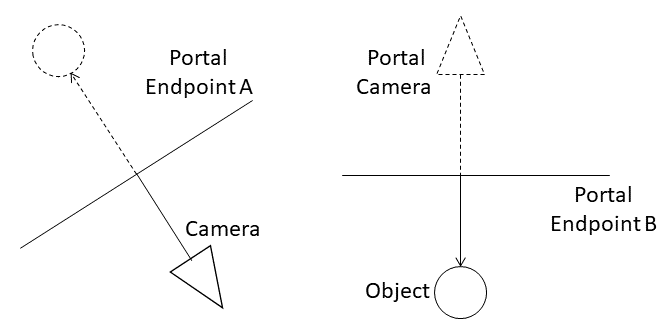
\includegraphics[width=\linewidth]{images/portal.png}
	\caption{A \gls{portalpair} connecting two parts of the world}
	\label{fig:portal}
\end{figure}

The connections of two parts of the world can be seen when looking at a portal. Figure \ref{fig:portal} shows the camera looking at endpoint A of a portal pair. It appears as if the dotted circle is in front of the camera. However, the actual circle is somewhere else. Instead of seeing endpoint A, the contents other part of the world is from portal camera's view point are seen.

\subsubsection{Teleportation Matrix 0.5}
To teleport objects travelling through portals their position and rotation need to be changed. Initially this was done by adjusting the location and rotations the following way: First the vector from an \gls{endpoint}['s] location to the the object is calculated. Then that vector is rotated by the rotation difference between the two endpoints. Finally that vector gets added to the other endpoint location. This is new position of the object origin. To calculate the portal view camera rotation, the original camera's rotation is multiplied by the rotation difference between the two endpoints. 

However the initial approach did only consider rotations and translations and was not really generic. A better way was devised using a \gls{teleportationmatrix}. When this matrix is applied to an object's \gls{modelmatix}, it is moved and rotated correctly. Additionally, the object is scaled by the difference in scale between the two end points. To transform an object first the \gls{endpoint} A's inverse \gls{modelmatix} is applied, after which \gls{endpoint} B's \gls{modelmatix} is applied. The \gls{teleportationmatrix} is just the product of those two matrices, so that operation can be performed in one step. \Gls{endpoint} B's teleportation matrix is the inverse of \gls{endpoint} A's \gls{teleportationmatrix}.



{\Huge Explainatin problems!!!}

Imagine an objects travelling through \gls{endpoint} A. Before relative transform to \gls{endpoint} A before the teleport must be equal to the relative transform to \gls{endpoint} B after the teleport. An objects modelmatrix expresses its transform realtive to the world. By multiplying the inverse modelmatrix of \gls{endpoint} A, \gls{endpoint} A's transform is subtracted from it. The object's transform is now relative to \gls{endpoint} A. This is the same realtive transform the object needs to

By applying the inverse of \gls{endpoint} A's \gls{modelmatix} to object's \gls{modelmatix}, the \gls{object}'s \gls{modelmatix} is now expressed relative to \gls{endpoint} A. If then \gls{endpoint} A's \gls{modelmatix} would be applied, the object would again be a the same position. However, by applying \gls{endpoint} B's \gls{modelmatix}, the \



The current approach uses coordinate transforms to calculate the portal view camera. By applying the inverse modelmatrix of endpoint A to the camera matrix, we bring the camera in a coordinate system, where endpoint A is at the origin. The camera matrix is now expressed relative to endpoint A. Finally we can apply Endpoint B's which moves exactly at the right position relative to endpoint B.
For example if the current camera's location where exactly at endpoint A, applying the inverse modelmatrix of endpoint A would move it to the origin.
The Application of the two matrices can be combined into one. The implementation this is called the teleportation matrix. It is also used to move objects from one end point to the other.  

%TODO other analogy? Relative attachments in scenegraphs? 





\subsection{Level}
A level represents the world and contains the \gls{portalset} and the \gls{objectset}.



\subsection{Camera 0.5}
In the implementation the user is able to move the camera in 6 directions, with key presses and rotate the view rotation with mouse movements. Additionally, the shift key can be pressed to lock the view direction, to readjust the mouse. Inputs are received via the \gls{sdl}'s \cite{sdl} \textit{SDL\_PollEvent} function.

The position is stored as a 3D point and the view rotation as quaternion. Position update take the camera's view rotations into account. Yaw rotations always rotate around the Y-Axis, while pitch rotation is relative to the current yaw rotation. Roll rotations are not supported.

With the position and rotation the \gls{cameramatrix} can be calculated. The inverse of this matrix is the camera's \gls{viewmatrix}, which is used for drawing from the camera's viewpoint.

\subsubsection{Perspective Matrix and Inverse Z-Buffer 0.25}
This implementation uses a perspective matrix with an infinite far clipping plane. Care needs to be taken, as Vulkan uses depth values from 0 to 1 \cite{khronos:vulkan:spec1.1} compared to open OpenGL's -1 to 1 \cite{khronos:openGL:spec4.6}. Additionally the implementation uses an inverse z-Buffer. An inverse Z-Buffer performs no worse than a regular Z-Buffer, but has improved accuracy when used with floating point depth buffers. For far away objects the depth distributions, becomes increasingly smaller. However, this values are also closer to and can make use a floating points increased precision near 0 \cite{lapidous:1999:optimal, nvidia:inversez}.


\subsection{Storing Mesh Data for Rendering}


\subsection{Portal drawing 5.75}
\label{section:portaldrawing}

This section covers various techniques used for portal rendering. How those techniques are actually applied will be explained in section \ref{section:intialimplementation}

\subsubsection{Recursions 0.33}
When looking through a portal the other part of the world can be seen. In that other part there can be another portal in which yet another part of the world can be seen. This could continue indefinitely, but in this implementation there is a limit. This limit is called the \gls{recursioncount}. A recursion count of 0, means that no other worlds can be seen through portals. A recursion count of 1 allows looking through portals, but portals at the other part of the world can not be looked through.

This implementation performs draws in multiple steps. Initially the initial world and the portals need to be drawn. This is referred as recursion 0. In within recursion 1 all the worlds for all visible portals from recursion 0 need to be drawn. Recursion 2 would draw the worlds for all portals drawn in recursion 1 and so forth. This continues until Recursion n, where n is equal to the \gls{recursioncount}.


\subsubsection{Textures vs Stencil Buffer 0.5}
\label{section:textursVsStencil}
Two different approaches were considered to render the contents of a portal. The first approach is to render the scene from the portal's viewpoint to a texture in the first renderpass. In the next renderpass this texture is applied to the portal and the whole scene is then rendered as usual \cite{lecture:portalProblems}.  %TODO: find source

The other approach utilises the stencil test. The stencil test is initially set to always pass. First only the \gls{objectset} is drawn. In the next renderpass the \gls{portalset} is drawn. For this renderpass, the stencil operation must be set in a way to mark the visible portal pixels. Now at least the depth values for visible portal pixels must be cleared. It is also possible to clear the whole buffer. Finally the scene is drawn again from the portal's view point. Fragments at pixel locations that are not marked are discarded. This ensures that it is only drawn to pixels where the portal was drawn \cites{schmalstieg:1999:sewing, lowe:2005:technique, lecture:portalProblems}.

For both approaches care must be taken to discard fragments that are between the portal's viewpoint and the portal exit. With multiple visible portals, the steps which use the portal's viewpoint, must be executed at least per visible portal. Additionally it must be ensured, that each portal has the correct contents.

This implementation uses the latter approach, as it does not need extra textures. Especially considering recursions, the first approach might need many textures and do not need the stencil buffer for anything else.

\subsubsection{Portal drawing orderer Depth first vs breadth first 1.25}

\begin{figure}[h]
	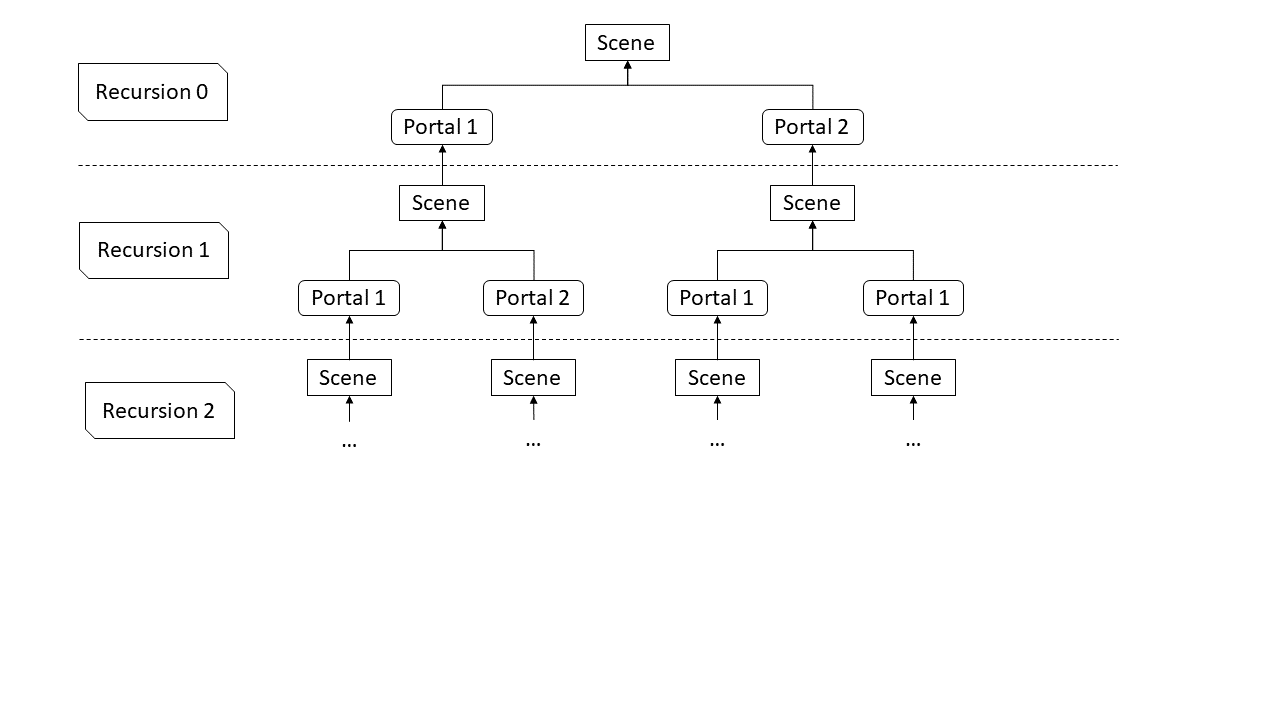
\includegraphics[width=\linewidth]{images/rendertree.png}
	\caption{Render Dependencies}
	\label{fig:rendertree}
\end{figure}


When drawing multiple portals recursively the draw dependencies can be imagined as a tree. Figure \ref{fig:rendertree} shows the dependencies for two portals. In recursion 0 the two portals can only be drawn after the scene was drawn. Otherwise portals that are occluded by a scene object might wrongly mark the pixel in the stencil buffer. The two scenes in recusion 1 can only be drawn when their respective portal was already drawn. However, it is not necessary that all portals from recursion 0 were drawn, before a scene from recursion 1 is drawn.

There are two approaches on the drawing order: depth first or breadth first. In depth first the contents of Portal 1 in recursion 0 would be fully complete, before it begins drawing the contents of Portal 2 in recursion 0. This has the advantage of needing just a small amount of different values to mark a pixel. Going down the tree a different value can be used for each recursion. When going up that value is not needed anymore and can be recyled. However, the implementation must make sure that no unneeded value remains in the stencil buffer. A downside is, that the draws are is fully dependent on each other.

Breath first draws a recursion completely before drawing the next recursion. The amount of different values needed to mark a pixel, scales exponentially. It needs one value of each portal in a recursion. For a scene with two portals, to mark all portals from recusion 1 it at least needs 4 different values, excluding 0. For recursion 2 it needs 8 values. With the stencil buffer usually being limited to 8 bits this can be quickly be a hard limit. However, the advantage is that the depth buffer needs to be cleared less often, only when transitioning between recursions. Additionally, within a recursion there are not dependencies between the multiple scene draws, as well as the portal draws.

Previous transformative portal implementations used depth first \cite{lowe:2005:technique,lecture:portalProblems}. The implementation presented in this thesis uses breadth first. Fewer dependencies between the draws could be exploited. Additionally similar draws can be grouped, which reduces the amount of renderpasses. While the amount of stencil values needed scales exponentially, the amount of draws scaled exponentially too. The author believes it is more likely that amount of draws will be the limiting factor than running out of values in the stencil buffer.



\subsubsection{Generating Camera Matrices 0.75}
As describe in section \ref{section:textursVsStencil} the scene needs to be rendered from the correct view point. This view point corresponds to the camera's view point teleported by the specific portal's \gls{teleportationmatrix}. As the camera moves the matrices must be calculated every frame.

\begin{figure}[h]
	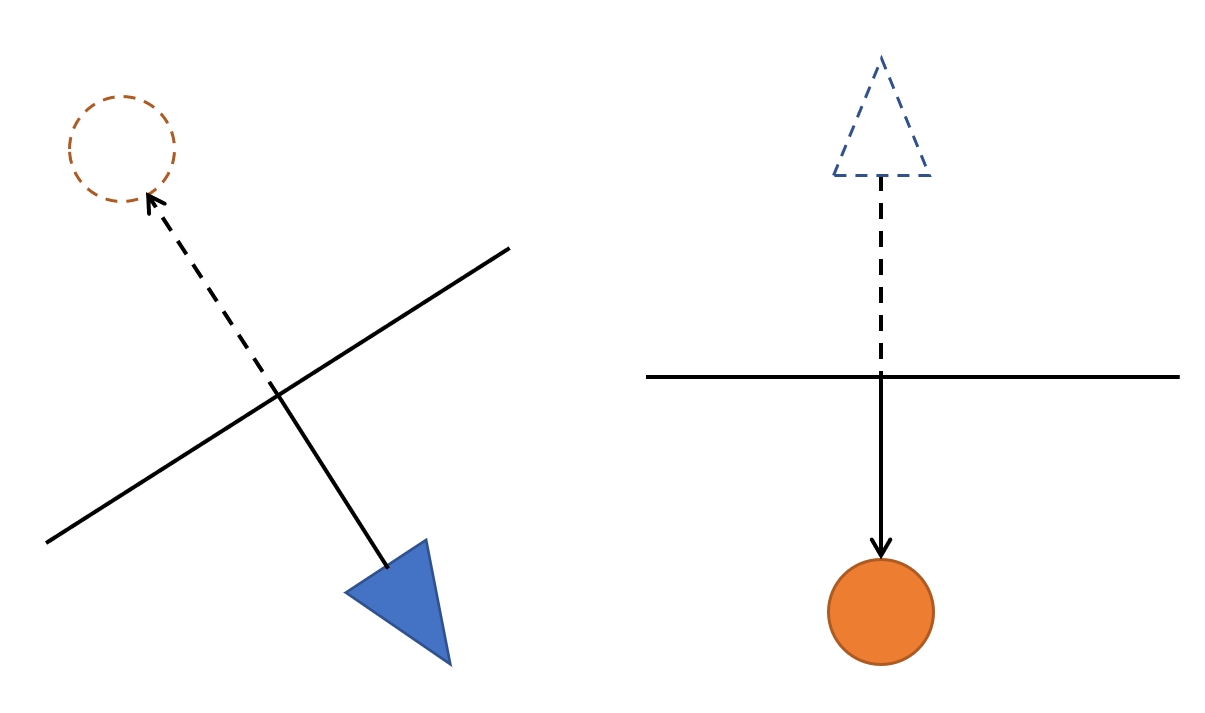
\includegraphics[width=\linewidth]{images/camera_matrices.png}
	\caption{Portal Camera}
	\label{fig:cameramatrices}
\end{figure}

Figure \ref{fig:cameramatrices} shows two portal endpoints. The blue triangle represents the camera and the orange circle represents an objects. The dotted blue triangle represents the portal view camera.
When looking through the portal, it must look as if the camera looks directly a the object. To move the camera to the correct location the \gls{endpoint}['s] \gls{teleportationmatrix} is be applied to the camera matrix. Then the  \gls{viewmatrix} can be obtained by inverting it.


\subsubsection{Recursive Portal Matrices 0.75}
\label{section:recursivecameramatrices}
The previous sections explained how to calculate the camera matrices for each portal for recursion 1. For recursion 2 a the camera's viewpoint must be transform twice, by two sequential applied \glspl{teleportationmatrix}. This needs to be done for every combination of two portals. For recursion 3 this is done for every combination of three portals and so forth. The implemtations stores the view matrices in a tree. The root is the current view matrix. An nth child node's matrix is equal to its parent matrix multiplied by the portal n's \gls{teleportationmatrix}. The tree is filled level by level.


The tree is layed out as an array and the indices can be found the following way:

\begin{itemize}
	\item $ nth child = current index * portalcount + 1 + n$
	\item $ parent = \lfloor(current index-1)/portal count\rfloor $
\end{itemize}



%%$c_n .. nth child index$
%%$p .. parent index$
%%$i ... curent index$
%%$t ... portal count$

\begin{figure}[h]
	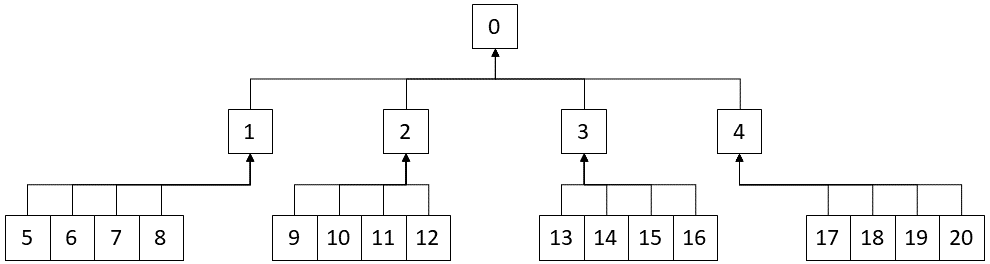
\includegraphics[width=\linewidth]{images/cameraindices.png}
	\caption{Camera Indices}
	\label{fig:cameraindices}
\end{figure}

Figure \ref{fig:cameraindices} shows the indices for 4 portals, with 2 iterations. For example to find the view matrix of Portal 0, seen through Portal 1, we would access the array at index 9. Note that the size of the three scales exponentially, with the \gls{portalcount} and \gls{recursioncount}, as every possible combination of portals needs to be covered. 


\subsubsection{Dual Depth Buffer 1}

When drawing the scene from the portals view, care must be taken to not draw objects, that are between the camera and other endpoint.
\begin{figure}[h]
	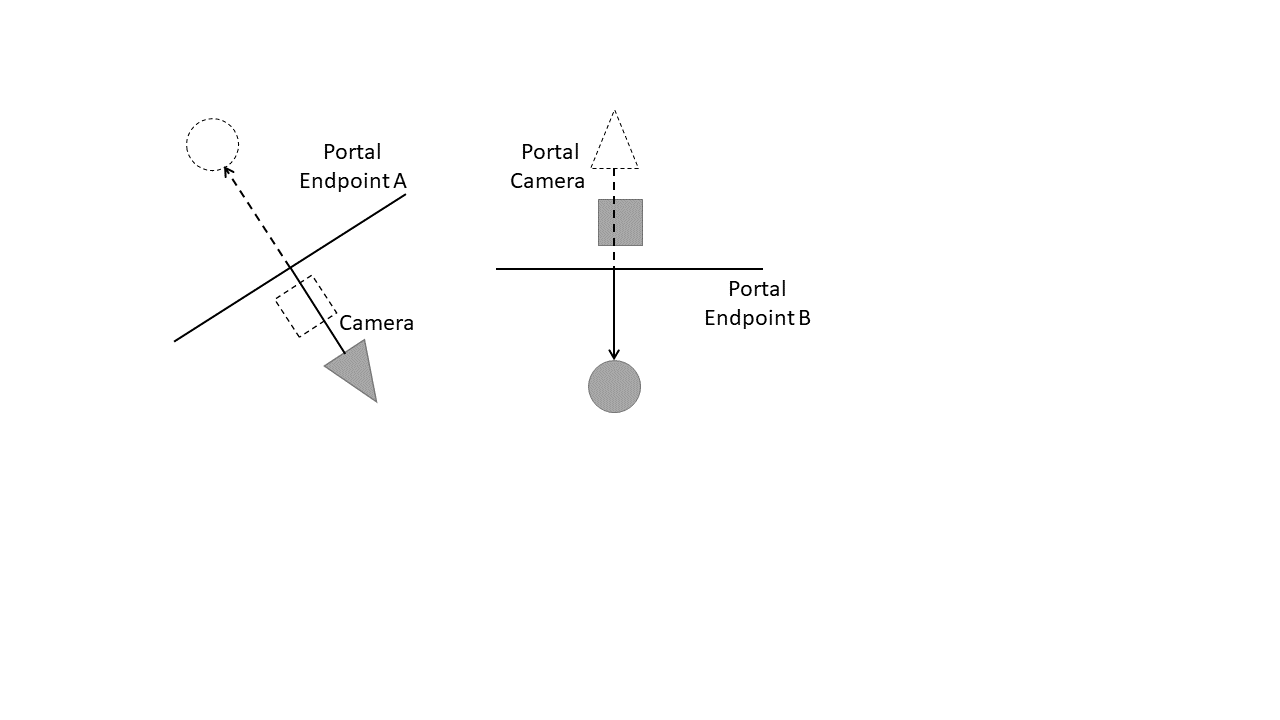
\includegraphics[width=\linewidth]{images/bananajuce.png}
	\caption{Object between portal camera and portal endpoint}
	\label{fig:bananajuce}
\end{figure}

Figure \ref{fig:bananajuce} shows such an example. Without additional techniques the square would be drawn. To avoid this, the implementation uses two depth buffers or dual depth buffer: a near depth buffer and a far depth buffer. The far depth buffer is used to discards fragments with a greater depth value. It is just a regular depth buffer, which is used in almost any rendering system. The near depth buffer discards fragments with a lesser depth value. When rendering the portal we render its depth also to the near buffer. The box's depth values from figure \ref{fig:bananajuce} would be greater than the near buffer and its fragments are discarded \cite{lowe:2005:technique}.

In this implementation the hardware supported depth buffer is used as the far buffer. For the near buffer dual buffering with two color texture are used, a read near buffer and a write near buffer. In the fragment shader, the fragments depth value is compared to the read near buffer. If it is lesser it is manually discarded, with a discard statement in the shader. Whenever the portals are drawn, they not only write the far depth buffer, but also the write near depth buffer. When the implementation transitions to the next recursion, the write near buffer and read near buffers are swapped.

Dual buffering the near buffer avoids problems with edge case where one portal occludes another and the portal behind is drawn first. With only one near buffer, the portal behind would set the near buffer to its value. The fragments of the portal in front would be discarded, instead of occluding the portal behind.

The read near buffer is a input attachment and the write near buffer is a color attachment. In recursion 0, no read near buffer test is used.

\subsubsection{Portal near Z fighting 0.33}
When rendering the contents of one endpoint of a portal pair, the other endpoint would be rendered directly at the same location. Due to precision errors in floating point calculations, the other endpoint would sometimes be discard by the near buffer and sometimes not. This leads to a special case of Z fighting. To avoid this we store the winding order of a fragment in the near buffer. When the fragments depth value and the near buffer value are nearly equal and winding order is the same, we have exactly the previously mentioned case and need to discard the fragment. This is done by increasing the comparison value by some small amount or percentage for same winding orders.

As the implementation has a depth range of 0 to 1, the value will always be positive. This allows the implementation to store the winding order is store as the sign of the near buffer. Positive values indicating front facing and negative values indicating back facing. Near Depth comparison is done with the absolute value of the buffer.

\subsubsection{Stencil Values and compare masks 0.66}
\label{section:stencilcomparemasks}

As the implementation uses the breadth first approach, it can not use the stencil increment and decrement technique described by other implementors \cite{schmalstieg:1999:sewing, lowe:2003:fragment, lecture:portalProblems}. Different values need to be stored and compared against. Directly setting the stencil value can be achieve, by setting a reference value and use the replace stencil operation. However, the stencil reference is also used for the comparison. This means that the implementation must be use the same value for comparison as well as writing. This can be achieved by the use of stencil compare mask and generating stencil values with postfixing.

\begin{figure}[h]
	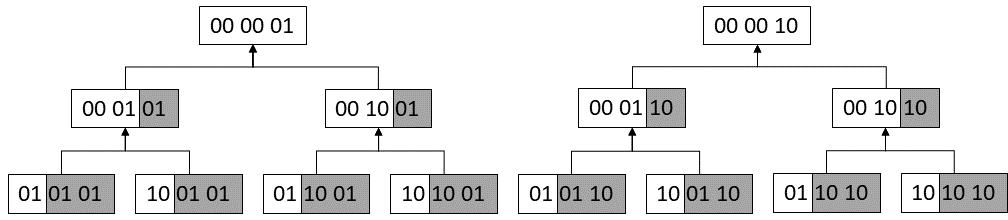
\includegraphics[width=\linewidth]{images/stencilvalues2.png}
	\caption{Compare Mask and Stencil Values}
	\label{fig:stencilvalues}
\end{figure}

Figure \ref{fig:stencilvalues} shows is process with two portals and 6 bits. The grey part is used for comparisions, while the whole value is used to write. The comparision mask of Recusion 0 mask out all bits, so the test will always succeed. For two portals recursion 1 mask out all but the last two bits. Notice that the last two bits of  recursion 1's stencil values are the same as their respective parent values. It is important that stencil values start with 1 and not with 0, otherwise they are not distinguishable from their parent values.

This also means that the range of values is one less than representable by the number of bits. This is very significant, as the portals come in pairs. The number of bits needed for two and four portals is one more than normally needed. As the stencil buffer usually only has eight bits, this limits the amount of recursions considerably.



\subsection{Initial Implementation 4.2}
\label{section:intialimplementation}
This section describes the first iteration of the implementation. It uses the specified techniques described in section \ref{section:portaldrawing} and focuses on how those are implemented.


\subsubsection{Renderpass Setup 1}
\label{section:renderpass}

The implementation uses just one renderpass, with multiple subpasses. This allows for the use of input attachments and potentially enables the \gls{gpu} driver to optimize. For example many textured are only needed within the renderpass and do not need to be transferred anywhere else.

\begin{figure}[h]
	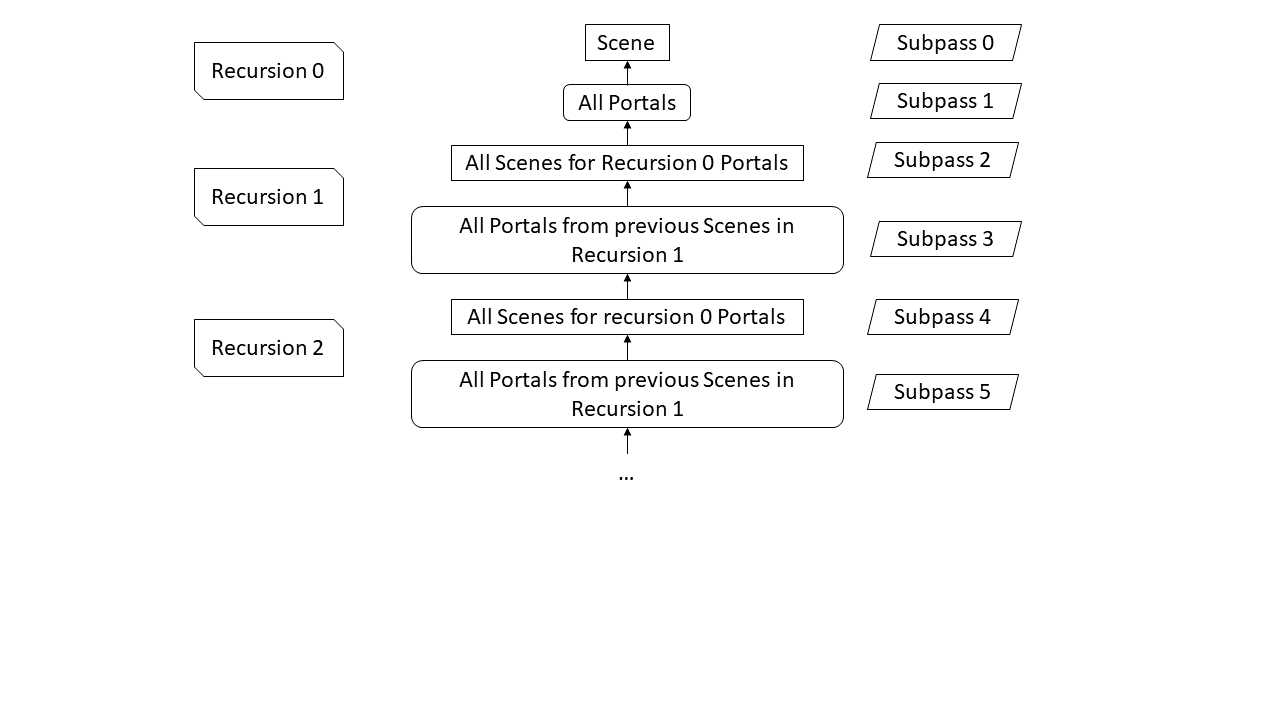
\includegraphics[width=\linewidth]{images/renderpasses.png}
	\caption{Subpasses and work done}
	\label{fig:renderpasses}
\end{figure}


Figure \ref{fig:renderpasses} shows the subpasses, which recursion they belong to and what work is done. Notice that compared to figure \ref{fig:rendertree} scene and portal draws are each batched together. Every even subpass is responsible for drawing a scene, while in every odd subpass the portals are drawn. The subpass index divided by two equals the recursion index. 

\begin{figure}[h]
	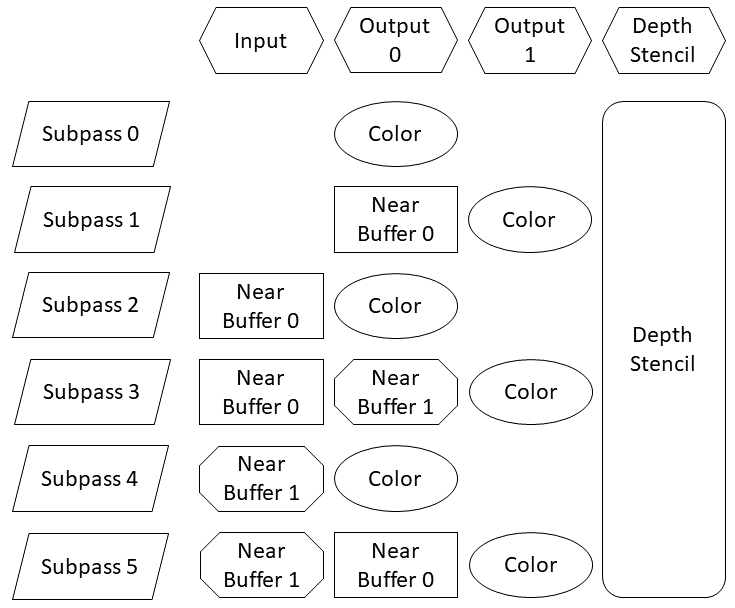
\includegraphics[width=\linewidth]{images/attachmentsetup.png}
	\caption{Attachment Setup}
	\label{fig:attachments}
\end{figure}

Figure \ref{fig:attachments} illustrates the attachments of the individual subpasses for two recursion. Odd subpasses write into the near buffer, which is used as input for the following two subpasses. For a real application portals do not need to write color so output 1 is not really needed. However, for this implementation it is kept for debugging purposes.
The last subpass does not need to write to the near buffer, as there are not later subpasses which could use it. It is kept for debugging purposes too. The depth stencil attachment is never changed. The color and depthstencil attachment are cleared at the beginning of the renderpass with VK\_ATTACHMENT\_LOAD\_OP\_CLEAR. Both near buffers use VK\_ATTACHMENT\_LOAD\_OP\_DONT\_CARE. The stencil test ensures that they are only accessed at locations where portals have previously written a value. Each subpass has set a dependency in the fragment shader on the previous subpass' output.


\subsubsection{Graphic Pipelines 1.5}
When rendering the multiple scene one after each other, as well as when rendering the portals, the stencil reference needs to be changed. There are two options how to resolve this problem: either using multiple pipelines or using dynamic pipeline state. For the implementation dynamic pipeline state was used, as the number of graphic pipelines needed would scale exponentially with the amount of portals and recursions. Dynamic state seemed much easier to manage in comparison.

However, the subpass index cannot be dynamic state. Thus even with dynamic stencil references, there must be at least the same amount of graphic pipelines as there are subpasses. If more than one shader is used for rendering scene objects or portals, the amount of graphic pipelines is increased. Each additional shader increase the amount by half of the subpass amount, as it is either only used for portal rendering or only for scene rendering. As there already are different pipelines for the subpasses, each of them can have a different stencil compare mask (see section \ref{section:stencilcomparemasks}). There is no need for dynamic stencil compare masks.

One important aspect is that pipelines for both scene and portal drawing, have face culling disabled. Portals do not have to be watertight and scene object might be transformed in a way that changes winding order. If it can be ensured that there are no teleportation matrices that change winding order, then face culling could be enabled for scene objects. For this implementation it was chosen to support such teleportation matrices.

The individual  graphic pipelines for drawing the scene differ by subpass index and stencil compare mask. This is also true for the graphic pipelines for portal drawing. Additionally, subpass 0 has the stencil test completely disabled, while subpass 1 uses an always succeeding test with VK\_STENCIL\_OP\_REPLACE. Other even subpasses use the stencil compare op VK\_COMPARE\_OP\_EQUAL with VK\_STENCIL\_OP\_KEEP for all test result. Other odd subpasses use VK\_COMPARE\_OP\_EQUAL with VK\_STENCIL\_OP\_REPLACE on stencil and depth test success, otherwise VK\_STENCIL\_OP\_KEEP

\subsubsection{Shaders 0.75}
Vulkan shader module requires the SPIR-V format. The shaders are written using GLSL and are compiled using the GLSL Validator (glslangValidator.exe). All fragment shaders contain the manual check with the near buffer. If it fails the fragment is discarded using the discard statement. However, for subpass 0 and subpass 1 there is no input attachement (see figure \ref{fig:attachments}). Those use shaders where the check is omitted. To prevent shader redundancies the shader is compiled twice. One of the compilations skips the check using the preprocessor and by command line arguments to the GLSL Validator. As previously mentioned in section \ref{section:renderpass} the portals drawn in the last subpass do not need to store anything in the near buffer. This could also be omitted using conditional compilation. All scene object only have one colour. It is passed via push constants. Additional minimal shading is performed using lambert shading with a fixed directional light.

Vertex shaders need to transform the vertices for all the different views. The different view matrices are stored in an \gls{ubo}. The index to access the current view matrix received via push constant. The model matrix is received also via push constant, as it changes per model and it there was still enough space in the push constant. The perspective matrix is passed via \gls{ubo}, as it never changes. Even if it would change than likely at most once per frame. The vertex shaders are the same for all scene draws as well as for all portal draws. No conditional compilation is needed.


The shaders are automatically recompiled after a change, using Visual Studio's Custom Build Tool feature. This enables fast iteration times, and avoids error due to forgetting to compile.

\subsubsection{Pre draw steps 0.25}

At the beginning it is waited on a fence to make sure, that submission of a previous command buffer has already finished. Then the fence is set to the unsignaled state. The camera matrices and perspective matrix are calculated. The result is written the respective \gls{ubo} via memory mapping and memcopy, as they use host visible memory. Their memory is also host coherent, so no explicit flushes are needed.
Then the next image from the swapchain is aquired. A semaphore is passed, which can be waited on before submitting the command buffer.
Lastly the the commandpool for the commandbuffer used for drawing is reset.

\subsubsection{Filling the command buffer 0.5}
The commandbuffer used for drawing was just reset via its commandpool in the pre draw steps. The first command is begin with a parameter indicating that this buffer is used for a one time submit. Then the renderpass is begun. Instanced drawing is not used so instance count is 1 and first instance is 0 for \textit{drawIndexed} calls.

Subpass 0 does not use the stencil buffer, so not reference needs to be set. Before drawing the scene \textit{bindIndexBuffer} and \textit{bindVertexBuffer} is called. All scene object vertices reside in the same buffer, so this only needs to be done once. Then for every object \textit{pushConstants} is called on the command buffer with the object specific push constants and \textit{drawIndexed}. 

To change to subpass 1, first \textit{nextSubpass} is called. Then, similar to supass 0, \textit{bindIndexBuffer} and \textit{bindVertexBuffer} is called.  Then for each portal the coresponding stencil value (see section \ref{section:stencilcomparemasks}) is set dynamically with \textit{setStencilReference}, then \textit{pushConstants} and finally \textit{drawIndexed} is called.

Subsequent even subpasses are similar to subpass 0, but the scene drawn is drawn multiple times. Each time with a different camera matrix id as push constant, as well as calling \textit{setStencilReference} with the different stencil values used in the previous subpass.

Subsequent odd subpasses are similar to subpass 1, but all portals are drawn multiple times. No portal has the same stencil value as any other portal.

The \gls{objectset} and \gls{portalcount} are drawn for each possible combination of portals. The amount a draws for each of them is equal to the size of the camera matrices array.


\subsection{Dynamic Portal Rendering 7.7}
One downside of the initial portal rendering strategy was its hard limit of total portals in the scene. No matter visible or not the portal was drawn and used up values in the stencil buffer. For two recursions, only 15 or less portals were allowed to exits in the scene. For three recursion only 7 or less, for four recursions only 3 portals were possible. For this reason a new method was derived which is limited by the visible portal count instead of the total portal count. 

When drawing a portal, it uses a stencil value depending on the number of visible portals drawn before it, instead of using a fixed value. However, this also means that the right camera index cannot be known before submitting.


\subsubsection{View Matrix Selection 1.66}
Except for subpass 0 and subpass 1, it is not known which camera index to access, as this depends on what portals were drawn previously. This problem is solved with an indirection.

\begin{figure}[h]
	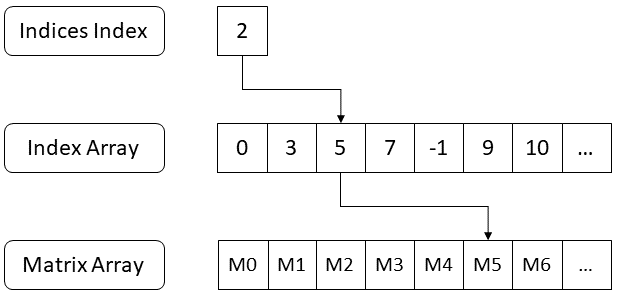
\includegraphics[width=\linewidth]{images/viewmatrixindirection.png}
	\caption{View Matrix Indirection}
	\label{fig:viewmatrixindirection}
\end{figure}

Figure \ref{fig:viewmatrixindirection} shows an example, how this works. Instead of receiving the index for the view matrix, an \textit{indices index} is received. The \textit{indices index} is used to access an element in an \textit{index array}. This element's value is the actual index, which is then used to find the correct view matrix in the \textit{matrix array}.

Sometimes there are less visible portals than the maximum count. This can not be known before submitting the command buffer. The draw commands for elements with non existing portals are still recorded in the command buffer. This implementation uses a special value -1 in the \textit{index array} to indicate such a case. It is an invalid index. The value of the view matrix index is the same for every vertex shader invocation of a mesh, as it depends on a push constant value. When encountering and invalid index as view matrix index, the vertex shader sets \textit{gl\_Position} to a fixed position. Every vertex of each triangle of an object, will have the same position. This results in all triangles being degenerate and they are culled \cite{khronos:vulkan:spec1.1}.

\begin{lstlisting}[caption={View Matrix Selection}, label=listing:viewmatrixselection]
// shader.vert
#version 450

...

layout(push_constant) uniform PushConstant {	
	mat4 model;
	int viewMatrixIndicesIndex
	...
} pc;

layout(set = 1, binding = 0) uniform Ubo_GlobalRenderData {
	mat4 proj;
} u_grd;

layout(set = 2, binding = 0) uniform ubo_cameraMats
{
	mat4 mats[maxCameraMatCount];
} u_cMats;

layout(set = 4, binding = 0) buffer ViewMatIndices {
	int vIndices[];
} vi;

layout(location = 0) in vec3 inPosition;

const int invalid_matIndex = -1;

void main()
{
	int viewMatIndex = pc.viewMatrixIndicesIndex == 0 ? 
		0 : vi.vIndices[pc.viewMatrixIndicesIndex];
	
	if(viewMatIndex != invalid_matIndex)
	{
		gl_Position = u_grd.proj * u_cMats.mats[viewMatIndex]
		 * pc.model * vec4(inPosition, 1.0);
	}
	else
	{
		// invalid index, create degenerate triangles
		// by setting every vertex to the same value
		gl_Position = vec4(1);
	}
	...
}

\end{lstlisting}

Listing \ref{listing:viewmatrixselection} shows the code of the vertex shader. Note that if the indices index is 0, it must be recursion 0. 0 can then be used as index for the camera matrices. This is convenient when filling the index buffer later.

\subsubsection{Properties of the Index Array 1.33}
\label{section:indexarrayproperties}

The implementation allows the max visible portal count to differ for each recursion. This is useful, as in recursion 0 the draw area is the whole screen, resulting in more visible portals. The contents within portals cover much less screen space, so it is less likely that portals can been seen within them. For each recursion the screen space drawn will get even smaller. This means recursion 0 will likely need the most visible portals, while the next recursion will need less and less visible portals.

\begin{figure}[h]
	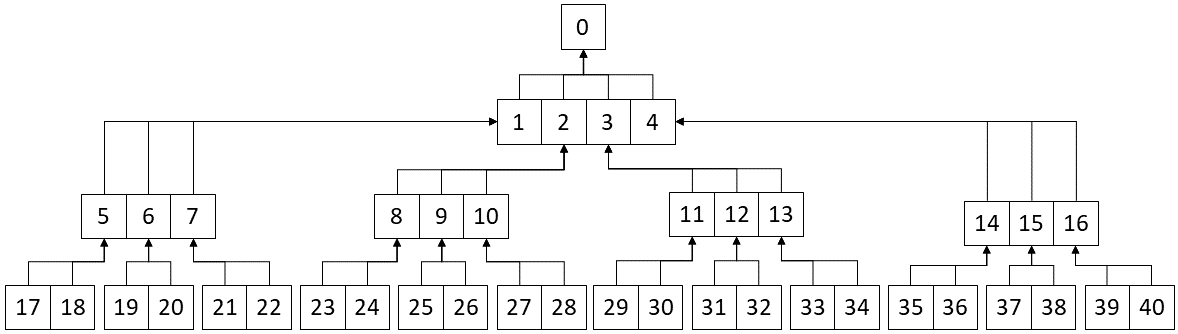
\includegraphics[width=\linewidth]{images/indexarray.png}
	\caption{Index array as tree for 4-3-2 visible portals}
	\label{fig:indexarray}
\end{figure}

Just as the view matrix array, the indices array is also a tree. However, due to the different amounts of visible portals for different recursions, it has a different amount of children in each level. Figure \ref{fig:indexarray} illustrates the connections between child and parent elements. The show tree supports 3 recursions. The visible portal count for the first recursion is four, for the second it is three and the third recursion it is two. The thee has one root. Each elements child count corresponds to its level in the tree.

The following terms are used for index calculation formulas
\begin{itemize}
	\item $L_n$ ... the nth level,
	\item $LC_n$ ... the element count of the nth level
	\item $LF_n$ ... the index of the first element of the nth level
	\item $LDC_n$ ... the number of direct child nodes for each element in the nth level. 
	\item $L_nE_i$ ... the index of the i-th element in the nth-level
	\item $L_nE_iC_k$ ... the index of the k-th child of the i-th element in the n-th level 
\end{itemize}

The following formulas can be used to calculate indices

\begin{itemize}
	\item $LC_0 = 1$
	\item $LC_n = LC_{n-1} * LDC_{n-1}$
	\item $LF_0 = 0$
	\item $LF_n = LC_{n-1} + LF_{n-1}$
	\item $L_nE_iC_k = LF_{n+1} + LDC_{n} * i + k$
\end{itemize}

For every recursion the whole corresponding level of the Index Array Tree is traversed, drawing each object and portal a total of $LC_n$ times. Using \ref{fig:indexarray} as example, every object and portal in recursion 0 is drawn 1 time. For recursion 1 is is 4 times, for recursion 2 its is 12 times. And Finally for the last recursion, recursion 3, everything is drawn 24 times. In total 41 draws would be issued for every object and portal.

\subsubsection{Filling the Index Array 1.33}
For the indirection from the previous section to work, the index array must be filled with correct values. Before starting to record draw commands, the index array is filled with an invalid index value by calling \textit{fillBuffer}. Listing \ref{listing:indicesindexcalculation} shows the algorithm used by the fragment shader to calculate and set the individual index array elements.

\begin{lstlisting}[caption={Calculating Indices Index}, label=listing:indicesindexcalculation]
// shader.vert
#version 450
...
layout(push_constant) uniform PushConstant {	
	int viewMatrixIndicesIndex;
	int maxVisiblePortalCount;
	int portalIndex;
	int maxPortalCount;
	int nextLevelStartIndex;
	int portalGroupIndex;
	...

} pc;

layout(set = 4, binding = 0) buffer ViewMatIndices {
	int vIndices[];
} vi;

void main()
{
	...
	int previousVisiblePortalCount = ...
	
	if(previousVisiblePortalCount < pc.maxVisiblePortalCount)
	{
		int currentViewMatIndex = pc.viewMatrixIndicesIndex == 0 ? 
			0 : vi.vIndices[pc.viewMatrixIndicesIndex];
		
		int firstPortalViewIndex = 1 +
			(currentViewMatIndex * pc.maxPortalCount);
		
		int currentPortalViewIndex = firstPortalViewIndex +
			pc.portalIndex;
		
		int firstViewIndicesIndex = pc.nextLevelStartIndex +
			(pc.portalGroupIndex * pc.maxVisiblePortalCount);
			
		int viewIndicesIndex = firstViewIndicesIndex +
			previousVisiblePortalCount;
			
		vi.vIndices[viewIndicesIndex] = currentPortalViewIndex;
	}
	...	
}

\end{lstlisting}

In each portals fragment shader the previous visible portal count is calculated. How this is done will be explained in the next section. It is then compared with the maximum visible portal count. If it the previous visible portal count is higher or equal to the maximum visible portal count the index array is not touched, by the shader.

If the previous visible portal count is less then the index for writing is calculated using $L_nE_iC_k = LF_{n+1} + LDC_{n} * i + k$ (see section \ref{section:indexarrayproperties}). $LF_{n+1}$ is provided by via push constant and is the same for the whole recursion.  $LDC_{n}$ is also the maximum visible portal count, which was used for the previous check. It is provided via push constant and also stays the same for the whole recursion. $i$ is equal to the number of previous portal groups for that recursion. It is provided via push constant and is increments for after each portal group. $k$ is equal to the number of previous visible portals, that was just calculated.

Now that the index for the element in the index array we want to write to has been calculated, the shader needs to write the right value to it. The portal that is currently drawn may be seen portal. Using the formula  $ nth child = current index * portalcount + 1 + n$ from section \ref{section:recursivecameramatrices} the view index can be calculated.  $currentindex$ was the index used in the vertexshader to access the right view matrix. The $portalcount$ is passed via push constants. $n$ is equal to the number of privious drawn portals in the portal group. It is also passed via push constants.

Every fragment shader invocation will either write the same value or write nothing at all. If no value was written to an index array element, its value will be the invalid index value. For the last portal iteration a visible portal count of 0 is passed, as indicator. That way the portals don't write outside the array.

\subsubsection{Visible Portal Number algorithm 1.5}
\label{section:visibleportalcount}
A portal is visible if at least one fragment of it was drawn. One commonly way of finding out if fragments were drawn are occlusion queries. Reading back the result of a occlusion to the \gls{cpu}, was deemed too slow. Although Vulkan also supports copying the result to a buffer by calling \textit{copyQueryPoolResults} on a command buffer, this is only possible outside of a renderpass. For this reason a different way of finding out, how many different portals are visible was derived.

The algorithm uses an helper array with integer elements and each drawn \gls{portalset} exclusively owns a range within it. No other group may read from or write to that range. This range is called \textit{Helper Range} The first index of the range is called \textit{First Helper Index}. The size of the range is equal to the \gls{portalcount}. Each portal in a group has an element within range, where it has exclusive write access. It is called \textit{Current Helper Element}. The index to that element is called \textit{Current Helper Index}. Before starting to draw the each element of the helper array is set to 0.

\begin{lstlisting}[caption={Calculate Previous Visible Portals}, label=listing:previousvisibleportals]
// portal.frag
#version 450
#extension GL_ARB_shader_stencil_export : enable

...
layout(push_constant) uniform PushConstant {	

int maxVisiblePortalCount;
int portalIndex;
...
} pc;

layout(set = 5, binding = 0) buffer PortalIndexHelper {
int indices[];
} pih;

void main()
{
...
int previousVisiblePortalCount = 0;
int currentHelperIndex = pc.firstHelperIndex + pc.portalIndex;

// stop at currentHelperIndex as we are not allowed to read it
// and the following elements were not written yet
for(int i = pc.firstHelperIndex; i < currentHelperIndex; ++i)
{
previousVisiblePortalCount += (pih.indices[i]) == 0 ? 0 : 1;
}

if(childNum < pc.maxVisiblePortalCount)
{
pih.indices[i] = previousVisiblePortalCount;
...
}
...
}
\end{lstlisting}

Listing \ref{listing:previousvisibleportals} illustrates the fragment shader algorithm. Each portal's fragment shader iterates from the \textit{First Helper Element} to the element before the \textit{Current Helper Element}. It increases a counter, each time the element is not zero.This count is equal to the number of previous visible portals and can be used for future calculations. Before drawing the next portal, a pipeline barrier is inserted, so that the writes of current portal's fragment shader are visible to the next portal's fragment shader.

This algorithm makes use of the property that if the fragment shader is never invoked, it will never write a value to its \textit{Current Helper Element}. If multiple shader invocations write the same non-zero value to the \textit{Current Helper Element} there will be that value, no matter how many invokation have written to it.
Thus if at least one fragment shader was invoke for the portal, there will be a non zero value at its position. As the element which is written to, is not read, the write does not influence the other shader invocations. The iteration does not need to continue after \textit{Current Helper Element}, as these values will not have been written yet and will always be 0.

\textbf{ \huge TODO: Ask Advisor if multiple same value writes trigger undefined behaviour? }%TODO: check for data race

The written value may can be any non-zero value, but writing the previous visible portal count allowed for easier debugging during the creation of the implementation.

\subsubsection{Properties of the Helper array 0.7}
The helper array and index array have a similar structure. For every element in the index array the \gls{portalset} is drawn. During the draw of one \gls{portalset} \gls{portalcount} elements in the index helper array are used. For the final last draw no indices need to be calculated, as nothing will be drawn after it. Thus the element count of the index helper array is equal to the element count of the index array, without its last level, times \gls{portalcount}.

\begin{figure}[h]
	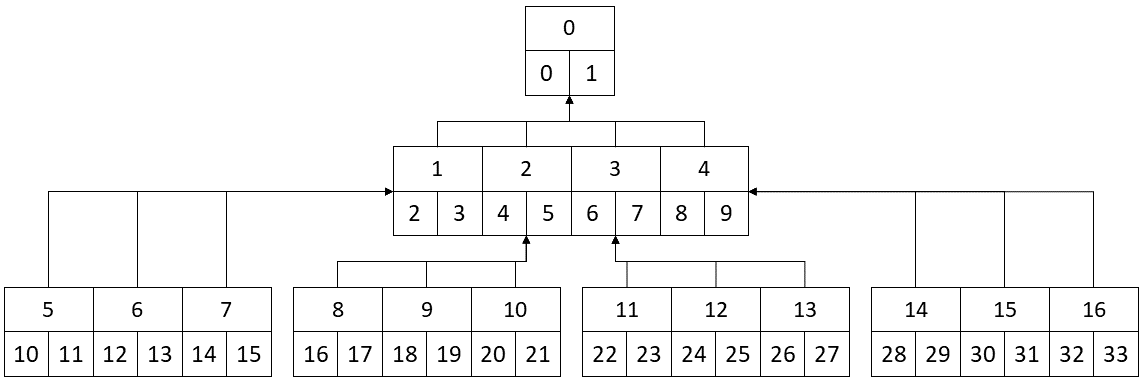
\includegraphics[width=\linewidth]{images/helperarray.png}
	\caption{Helper array as tree for 4-3-2 visible portals, with \gls{portalcount} of 2}
	\label{fig:helperarray}
\end{figure}

Figure \ref{fig:helperarray} shows the helper array as tree, with a \gls{portalcount} of 2. It uses the same recursion count and visible portal count as the index array of figure \ref{fig:indexarray}. The top number in the bigger rectangle corresponds to the index helper tree for easier comparison. Notice that the first index of the actual elements in the bottom boxes is equal to are the top number times the \gls{portalcount}. This first index corresponds to the individual \textit{First Helper Indices}. The same formulas as described in section \ref{section:indexarrayproperties} can be used to calculate those indices. They first need to be divided by the \gls{portalcount}, then used in the formula and the result multiplied by \gls{portalcount}.


\subsubsection{Calculating the Stencil Reference 0.9}
Before drawing it is not known how which and how many portals are actually visible. The stencil value cannot be set dynamically when recording the command buffer. Instead the stencil reference is calculated in the shader and set via the Vulkan extension VK\_EXT\_shader\_stencil\_export. As this is an extension this feature is not supported on every \gls{gpu}.

\begin{lstlisting}[caption={Calculate Stencil Reference in Shader}, label=listing:stencilcalculation]
// portal.frag
#version 450
#extension GL_ARB_shader_stencil_export : enable

// ...
layout(push_constant) uniform PushConstant {	
	uint parentStencilReference;
	int stencilReferenceBits;
	int maxVisiblePortalCount;
//...
} pc;

out int gl_FragStencilRefARB;

void main()
{
	...
	int previousVisiblePortalCount = ...
	
	if(previousVisiblePortalCount >= pc.maxVisiblePortalCount)
	{
		...
		uint myStencilReference = previousVisiblePortalCount + 1;
		uint stencilReference = pc.parentStencilReference 
		| myStencilReference << pc.stencilReferenceBits;
		gl_FragStencilRefARB = int(stencilReference);
	}	
	...
}
\end{lstlisting}

Listing \ref{listing:stencilcalculation} illustrates the calculation. The current stencil reference is passed via push constants. This is the same reference for the whole portal group. The fragement shader calculates the current visible portals and adds 1 to it, as using 0 as stencil reference would lead to ambiguities (see section \ref{section:stencilcomparemasks}). That stencil reference needs to be shifted by the amount of bits used by parent stencil reference and then ORed together. Shifting is done using unsigned types to avoid potential undefined behavior.

\subsection{Dynamic Portal instance rendering 1.25}
Dynamic Portal Rendering moved the limit from maximum portals in a scene to maximum visible portals, while also improving performance a bit. However, the performance was still pretty bad. Occluded portals or portals failing the stencil test still counted as beeing visible. This is due to the late stencil depth test, which was needed for the stencil export.

Additionally, every object and portal is drawn many times for all the visible portals and recursion. Trying to take advantage of that fact was not trivial. Although, it is possible to draw multiple instances of an object, it is not possible to change the stencil reference between each draw. Using stencil export for scene objects, would have gotten rid of the early fragment test. The only other way was to drop the stencil test, and perform a manual stencil test, similar as already done with the near buffer. After trying out that manual test and seeing not much performance penalty, the author decided to work try out instanced rendering.

Most changes to the code were transforming transforming the loops. Listing \ref{listing:looptransform} shows the difference in pseudo code.

\begin{lstlisting}[caption={Pseudocode Loop Transformation}, label=listing:looptransform]
// old 
for(int i = 0; i < previousPortalCount; ++i)
{
	commandBuffer.setStencilRefrence(stencilReferences[i]);
	for(int k = 0; k < sceneObjectCount; ++k)
	{
		commandBuffer.pushConstants();
		commandBuffer.drawIndexed(sceneObjects[k], 1);
	}
}

// new
for(int i = 0; i < sceneObjectCount; ++i)
{
	commandBuffer.pushConstants();
	commandBuffer.drawIndexed(sceneObjects[i], previousPortalCount);
}
\end{lstlisting}

Calculating the stencil references can be simplified. Using the same stencil reference to compare and set the stencil buffer is no longer needed. The stencil reference values nows increment by one for each instance. In fact the stencil reference value and indices index is the same. The indices index for the first instance is passed via push constants. The shaders can calculate their current \textit{indices index} and stencil reference by adding gl\_InstanceIndex to it.

The portal shaders use the gl\_InstanceIndex instead of the portal group id. The multiple instances of the same portal, all use a different range in the helper index array. They don not interfere with each other. As there is no synchronisation needed between the instances they can all use instance drawing and have their draw loop transformed similar to the scene objects. However, Pipeline barriers between are still needed between drawing different portals.

The \textit{First Helper Index} is equal to the stencil reference/\textit{indices index} times the total portal count. {\huge explain better!} %TODO explain better

Changing the code to use instance drawing, resulted in a huge performance increase. Compared to the previous version, the code was 6 times fast on a particular configuration. Additionally, doing the manual stencil test, allows earlier fragment shader discards, reducing the amount of false visible portals. Furthermore, the stencil export extension is no longer required, so the application can run on more graphic cards. Finally, the texture used for the manual stencil test can be bigger than a real stencil buffer. This effectively removes a hard limit of the maximum visible portals count and recursion count. Those are now only limited by computation speed.


\subsection{Portal Collision 0.75}
One important aspect of portals is actually moving objects. Without further work, the portals on teleport the view. For this implementation teleporting was implemented only for the camera, as a proof of concept.

\subsubsection{Collision Detection 0.25}
The camera is imagined as an object without volume. Each time the camera is moved a ray cast is performed from the camera's old location to its new location. The ray intersection is first performed against the portals' \glspl{aabb}. For the test a the method described by \textcite{williams:2005:efficient} was used. If the test passes the ray is tested the portals mesh's triangles using the triangle intersection algorithm described by \textcite{moller:2005:fast}.


The triangles and bounding box are store in the model space coordinates. This way only one triangle mesh and bounding boxed needs to be stored for portals using the same model. Before a the ray is tested against bounding box and triangles it needs to be transformed into model space. This is achieved by applying the portal's inverse model matrix to the ray.

\subsubsection{Collision Response 0.25}

After a collision the camera needs to be moved to the correct location. The process is the same as the one used to calculate the view point (see section \ref{section:recursivecameramatrices}). However, this matrix can not be directly applied, as the cameras position and rotation are not stored in matrix form.
And additional matrix was added to the camera object, called \textit{additional transform}.

Whenever the camera's position, rotation or camera matrix is needed, they are first modified by the \textit{additional transform}. \textit{Additional transform} is initially equal to the identity matrix. Whenever portal collision occurs, the portal's teleportation matrix is applied to the \textit{additional transform}.



\subsection{Camera Object Rendering 0.2}
When looking through a portal the camera should see itself. However, always rendering the camera results in seeing itself from inside. The implementation avoids this problem, by only conditionally drawing the camera mesh. In the first sub pass drawing the camera is skipped. It is only drawn for subsequent passes.


\subsection{Level Editor 0.5}
To build level some kind of level editor is needed. Imagining the level only in the mind and writing the objects transformation directly into a file, is very difficult and time consuming.

Ideally a custom level editor should be built, so the effect of the portals can be seen immediately. However, there was not enough time and other parts of the implementation were prioritised. After looking for various solution, using the \gls{ue4} \cite{ue4} seemed best, as the author of this thesis has some experience with it.The \gls{ue4} Editor is very convenient to use and can be customized. Additionally, code can be executed within the editor, which can query level data.

An additional object type was added to editor, which was used placing the portals in the level. A small script was written to export the levels. It queries for all objects and portals in the level and stores that information in an XML file using RapidXml \cite{rapidxml}. Additionally all meshes from objects in a level are exported as OBJ by the script. However, some care must be taken as UE4 has a different coordinate system. For Vectors Y and Z must be swapped. For Quaternions, y and z must be swapped and the imaginary part inverted, as the handedness was changed.


\section{Analysis And Improvements 0/15}

\subsection{Swap Near Buffer with far Buffer}


\subsection{Visible Portal count}

in fragmentshader: counter, traverse array, increase for non zeros, ignore at index corresponding to the current portal
write own number or 1 at the ignored location -> Multiple writes of same value should be save, accross "threads", when counting this is skipped so we have no reader at the moment
Needs synchornisation so that value is visible for the next portal!
-> Pseudo occlusion query with immediate result.
-> very conservatic. Portals totaly occluded by later portals or discarded by stencil test still counts as "visible". We can't check for stencil failure, as we can't access the stencil buffer.
-> depth prepass could mitigate this

\subsection{GPU Raytracing}

\subsection{Camera Matrix Improvement opportunities}
Could be improved. The work to calculate the matrices scales super linear. $X^{N}$, where X is the portal count and N is the number of iterations.
Instead of precomputing all combinations, it is probably better to calculate the matrices on demand in the fragment shader, as we have much more information there. This saves unnessary computes, removes an indirection and puts the work on the gput. Only downside is that the computation is executed multiple, once per shader fragment. Finally save on bandwith, as they don't need to be transfered!


Dont actually need to be computed every frame, if additional matrix multiplications are ok.
Multiplying only the inverse matrices! but from the other side!


\subsection{Scaling measurement}

\subsection{Watertight Portals}
Objects behind watertight portals, will look as though that portal did not exist. Portals inside on endpoint of an watertight portals, will be visible when looking at the other endpoint, with the teleportation matrix applied. If watertight portals are static, they are essentially useless. The same scene could have been created without them.
However if they change or are created during runtime they can have interesting effects. Such as Scaling objects, or swapping two areas.

\subsection{Dynamic Portals Instance Rendering}

\subsubsection{Opportunity: Dynamic Visible Portals count}
If we can detect the initial pass only has few visible portals (e.g. via frustrum culling like techniques), we lower the amount for the initial rendering, and increase it for
the subsequent pass.

Handles case of directly standing in front of a portal!
Have not implemented this

\subsubsection{Opportunity: Draw Indirect}
Using draw Indirect allows us to only use one draw call per pass, instead of one per object!
Additionally we can manipulate the draw indirect buffer, while calculating the portal id, so that the instance count matches the amount of actually drawn portals.
This way instead of producing degenerate triangles, we don't even draw meshes.
However, could be problematic as we would need to set each value in the shader, having a loop for each scene element, and many writes.

The conditional execution extension could be used (VK\_EXT\_conditional\_rendering) but only to disable drawing entirely, if no portal is rended -> probably not useful.

\subsubsection{Skip instances}
One downside is, that draw instanced draws the object for each portal. However sometimes would could know, that the object is not visible from a specific Portal, e.g. via Potentially visible set tests, or knowing by other means that the portal will never draw that object (e.g. diffrent world layers).
To combat this problem, we could decrease the draw instances count and provide iformation which portals should be skipped.

Instead of using instanceId directly, this skip information will be used to calculate the real id. The rest would behave the same, just using this genreated id instead of instanceId directly.



\subsection{Non-Translating Portals}
The implemented portals have two endpoints. Objects Touch on endpoint, get move to the other. However, it is also possible that the portals don't move the object. In this case there are no two end points. It is just one portal.

Entering the portal would apply one operation (e.g. multiplying by matrix), leaving it applies the inverse operation. Back and Frontface detection needs to be used to decide which operation to apply.


This only works for operations which don't move the possition of an object, unless it is just an rotation and the portal shape looks the same after applying the rotation to it. E.g. a sphere could allow for any rotation. A cube only for rotation in intervals of 90 degrees.
Changing the scale of an objects would also work, but it is important, the the origin remains a the same position. However, this would result in non seamless portal transitions.

Furthermore, more than just transform can be applied. Operations described in the section \ref{more than transforms} would also work.

\subsection{Objects touching portals}

 The camera object should be able to see itself


When looking through a portal, players might see themselves. Care must be taken when rendering. Standing directly in fron of the portal and touching it slightly could make the player see their only model at their own location. (see valve talk \url{https://www.youtube.com/watch?v=riijspB9DIQ})
\subsection{Part translation}


On portal collision we apply the same operation on the camera, that would be applied to an object rendered through that portal.
It is implemented by storing a matrix of cumulative portal teleport matrices.
However, it is also possible to apply only a part of it for some interesting effects, but it will result in non seamless translation.

\section{Further Work 0/5}
\subsection{Transparent Objects}
\subsection{Shadows}
Without currect handling, we can see portal locations, as shadows would be cut of.
\subsection{lighting}
Without correct lighting seams would be visible. Proabably very difficult for spot/pointlights. Directional light already works.
\subsection{Collision Detection}

\subsection{More than just transforms}
\label{more than transforms}
The current approach uses camera indices, to decide which camera matrix gets applied. However, this approach is not limited to only changing matrices. Inspired by \cite{borst:2009:real} indices could be used to change other paramteres. We could add objects that only render if specific parameters are set, mark pixels for a later post process. Or take as specific branch in any shader.


\subsection{Use the Instant Occlusion query in occlusion culling}
we can set conditional rendering paramters during this occlusion culling.
Needs some  recursive portal passes and then one big scene pass, which makes use of conditional rendering, eitehr with the extension or draw indirect and instance counts. Inspired by \cite{yang:2014:walkthrough}

\section{Conclusion 0/3}

summary
instant pseudo query and other important topics
economic effekt

\section*{stuff}
For debugging OpenGL offers debug output to obtain details about errors, performance warnings and other useful information. They can be obtained via a debug message callback or by querying them from a message log \cite{khronos:openGL:spec4.6}. In Vulkan validations layers are used for finding errors. In Vulkan \gls{api} calls can be intercepted by layers. They perform whatever operation defined by their implementation before maybe passing them to the actual function. Validation layers are layers w

They validate the parameters, before passing them to the actual function. How errors are reported depends on the implementation of the layer.. Multiple layers can be active and are called each one sequentially before calling the actual function. \cite{khronos:vulkan:spec1.1}












